\section*{Question 2 --- DC motor with quadratic drag}
\answer{(a) State-space model}
Let $x_1=\theta$, $x_2=\omega=\dot\theta$ and $x_3=i_a$, with armature voltage $u$ and output $y=\theta$. Then
\begin{equation}
x=\begin{bmatrix}\theta\\\omega\\i_a\end{bmatrix},\qquad
\boxed{\dot x=
\begin{bmatrix}x_2\\\frac{K_Tx_3-d_1x_2-d_2x_2|x_2|}{J}\\-\frac{K_ex_2+R_ax_3}{L_a}\end{bmatrix}
+\begin{bmatrix}0\\0\\1/L_a\end{bmatrix}u},\qquad
y=\begin{bmatrix}1&0&0\end{bmatrix}x.
\end{equation}
The Simulink plant has three Integrators and separate mechanical/electrical equations; the closed-loop block diagram is shown in Appendix~A.

\answer{(b) Input-output linearization, new states and validity}
Define $\alpha=(K_Ti_a-d_1\omega-d_2\omega|\omega|)/J$ and $D(\omega)=d_1+2d_2|\omega|$. Since $\frac{d}{d\omega}(\omega|\omega|)=2|\omega|$, including at zero,
\begin{equation}
\dot y=\omega,\quad\ddot y=\alpha,\quad
y^{(3)}=-\frac{K_T}{JL_a}(R_ai_a+K_e\omega)-\frac{D(\omega)}{J}\alpha+\frac{K_T}{JL_a}u.
\end{equation}
Thus the linearizing voltage is
\begin{equation}
\boxed{u=R_ai_a+K_e\omega+\frac{L_a}{K_T}\bigl[Jv+D(\omega)\alpha\bigr]}
\quad\Longrightarrow\quad y^{(3)}=v.
\end{equation}
Choose $z=[\theta,\omega,\alpha]^\mathsf{T}$; then $\dot z_1=z_2$, $\dot z_2=z_3$, $\dot z_3=v$. Its inverse is $i_a=(Jz_3+d_1z_2+d_2z_2|z_2|)/K_T$. For $J,L_a,K_T>0$, the input coefficient $K_T/(JL_a)$ and coordinate Jacobian determinant $K_T/J$ never vanish. The law is globally defined for finite ideal-model states, including speed reversal. The transformation is $C^1$; there are no internal dynamics.

\answer{(c) Reference tracking: approximately 0.2 s settling}
For a constant reference $r=\theta_d$, choose
\begin{equation}
v=k_1(r-z_1)-k_2z_2-k_3z_3.
\end{equation}
The error $e=r-\theta$ satisfies $e^{(3)}+k_3\ddot e+k_2\dot e+k_1e=0$. Matching its polynomial to $(s+\lambda)^3$ gives
\begin{equation}
\boxed{k_1=\lambda^3,\qquad k_2=3\lambda^2,\qquad k_3=3\lambda.}
\end{equation}
From rest, $e(t)/e(0)=e^{-\lambda t}[1+\lambda t+(\lambda t)^2/2]$. Choose $\lambda=\tau_\varepsilon/T_s$, where $e^{-\tau_\varepsilon}(1+\tau_\varepsilon+\tau_\varepsilon^2/2)=\varepsilon$. For $\varepsilon=0.02$ and $T_s=0.2$ s, select $\lambda=38$ s$^{-1}$, yielding $k_1=54872$, $k_2=4332$, $k_3=114$ and predicted settling of 0.198 s. For smooth moving references, add $r^{(3)}+k_3\ddot r+k_2\dot r$ to the control law.

\answer{(d) Closed-loop simulation}
For simulation, use $J=0.01$, $K_T=K_e=0.2$, $R_a=2$, $L_a=0.05$, $d_1=0.01$ and $d_2=0.005$ in the supplied SI units. The input coefficient becomes $K_T/(JL_a)=400$. Acceleration is calculated from speed and current. From zero state, the reference steps to 0.1 rad at 0.05 s. The simulation runs for 0.5 s using \texttt{ode45}, maximum step 0.0005 s and relative/absolute tolerances $10^{-8}/10^{-10}$.
\begin{center}
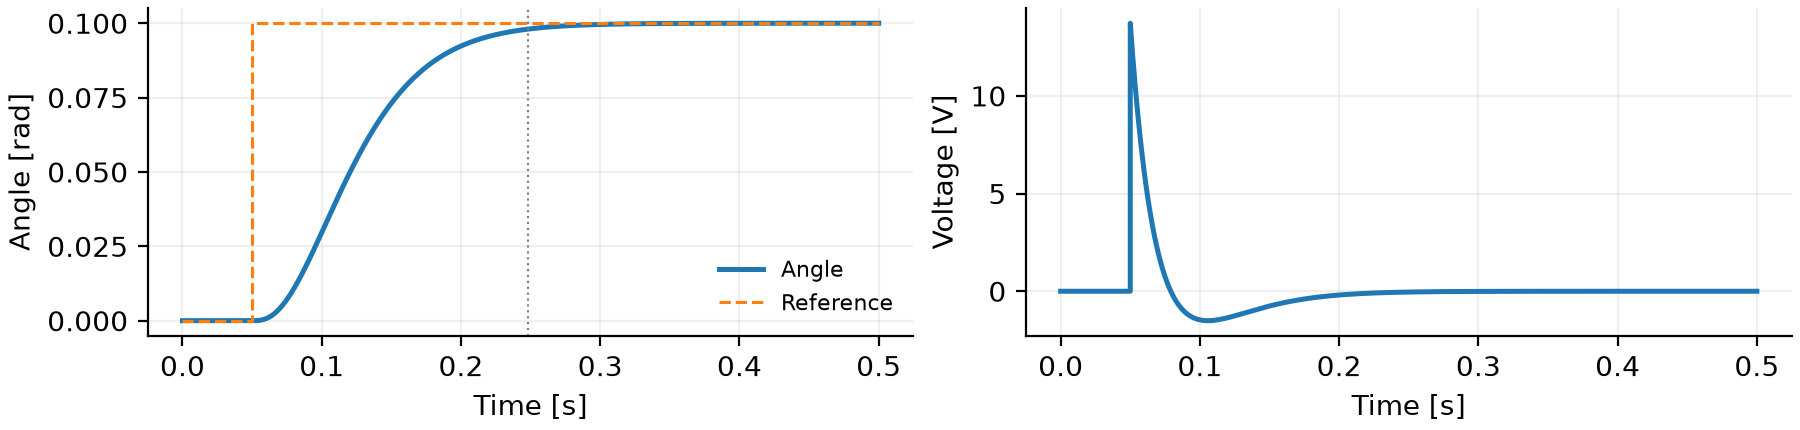
\includegraphics[width=\linewidth]{report_dc_motor_tracking.png}
\reportcaption{Simulated position tracking and applied voltage. Settling time is measured from the reference step.}
\end{center}
The measured 2\% settling time is \textbf{0.198 s}, meeting the approximate 0.2 s requirement, with no overshoot. Peak voltage is 13.718 V for the 0.1 rad step. Six cases check signed references, different initial states, the analytical closed-loop response and the exported model. Larger commands require larger voltage (27.436 V for a 0.2 rad step); no actuator limits or hardware feasibility are assumed.

